% Complete finite-difference lesson, included at the first introduction.
\topic{7}{Finite differences: from a slope to a formula}\label{sec:fd-slope}
A computer stores finitely many samples of a continuous field. Finite differences turn derivatives into algebraic combinations of these samples. We derive the formulas, measure their errors, and assemble a Poisson equation.

Use a uniform grid $x_i=x_0+ih$, with $h=x_{i+1}-x_i$, $f_i=f(x_i)$, and $f'_i=f'(x_i)$. A prime means differentiation, not an iteration. A derivative is a limiting slope, $f'(x_i)=\lim_{h\to0}[f(x_i+h)-f(x_i)]/h$. On a grid, $h$ is finite. We approximate the derivative using available samples and ask how the neglected terms depend on $h$. A difference is the numerator; a derivative approximation also divides by the correct distance.

\begin{center}
\begin{tikzpicture}[x=2.4cm,y=1cm,>=stealth]
\draw[->] (-.35,0)--(2.5,0) node[right] {$x$};
\foreach \x/\lab in {0/{i-1},1/i,2/{i+1}}{
\fill[accent] (\x,0) circle (2pt);
\node[above=5pt] at (\x,0) {$f_{\lab}$};
\node[below=5pt] at (\x,0) {$x_{\lab}$};}
\draw[<->] (0,-.9)--(1,-.9) node[midway,below] {$h$};
\draw[<->] (1,-.9)--(2,-.9) node[midway,below] {$h$};
\end{tikzpicture}
\end{center}
\textbf{What is a Taylor expansion?} It approximates a smooth function near $x_i$ by a polynomial. The term $hf'_i$ predicts change using the slope; $h^2f''_i/2$ corrects for curvature. The remainder $O(h^4)$ is bounded by a constant times $h^4$ for small $h$ and bounded higher derivatives. Expanding on both sides gives
\begin{align*}
f_{i+1}&=f_i+h f'_i+\frac{h^2}{2}f''_i+\frac{h^3}{6}f'''_i+O(h^4),\\
f_{i-1}&=f_i-h f'_i+\frac{h^2}{2}f''_i-\frac{h^3}{6}f'''_i+O(h^4).
\end{align*}
Subtract $f_i$ from the first line and divide by $h$:
\[
f_{i+1}-f_i=hf'_i+\tfrac12h^2f''_i+\cdots
\quad\Rightarrow\quad
\frac{f_{i+1}-f_i}{h}=f'_i+\tfrac12hf''_i+\cdots.
\]
The second expansion gives the backward formula; subtracting the expansions gives the centered formula. Error below means approximation minus exact derivative:
\begin{center}\begin{tabular}{lll}\toprule
Method & Approximation to $f'_i$ & Leading error\\\midrule
Forward & $(f_{i+1}-f_i)/h$ & $+(h/2)f''_i$\\[5pt]
Backward & $(f_i-f_{i-1})/h$ & $-(h/2)f''_i$\\[5pt]
Centered & $(f_{i+1}-f_{i-1})/(2h)$ & $+(h^2/6)f'''_i$\\\bottomrule
\end{tabular}\end{center}
\textbf{Why $2h$?} The centered numerator spans from $x_i-h$ to $x_i+h$, a distance $2h$. Dividing it by $h$ would double the derivative.

\textbf{Why use the centered formula here?} For smooth interior fields with values on both sides, symmetry cancels the $O(h)$ term. The resulting $O(h^2)$ error is the reason for choosing it in this introductory diffusion and Poisson discretization. It does not guarantee stability for advection-dominated flows or shocks; a complete time-dependent scheme must also satisfy stability and boundary requirements.

\textbf{Boundary distinction.} At $i=0$ there is no stored $f_{-1}$. A centered stencil therefore needs ghost values or a different boundary formula. A second-order one-sided derivative is $(-3f_0+4f_1-f_2)/(2h)$. For cavity walls, Section~8 derives the boundary treatment.
\checkpoint{Which approximation needs the center value $f_i$, and which needs both neighbors? Do not confuse the first derivative with the three-point second derivative in Section~7.1.}
\newpage
\topic{7.1}{Worked examples: accuracy and curvature}\label{sec:fd-errors}
Take $f(x)=x^3$ at $x=1$. The exact slope is $f'(1)=3$. For $h=0.1$, the samples are $f(0.9)=0.729$, $f(1)=1$, and $f(1.1)=1.331$:
\[
D_+f=\frac{1.331-1}{0.1}=3.31,\quad
D_-f=\frac{1-0.729}{0.1}=2.71,\quad
D_0f=\frac{1.331-0.729}{0.2}=3.01.
\]
\begin{center}\begin{tabular}{rrrrr}\toprule
$h$ & Forward & Backward & Centered & $|D_0f-3|$\\\midrule
0.10 & 3.3100 & 2.7100 & 3.0100 & 0.0100\\
0.05 & 3.1525 & 2.8525 & 3.0025 & 0.0025\\\bottomrule
\end{tabular}\end{center}
Halving $h$ reduces the centered error by a factor of four here. This is what second-order truncation error means: approximately $C h^2$ for a smooth fixed function as $h$ decreases. It does not mean two decimal places or two iterations. At extremely small spacing, roundoff and subtractive cancellation can become important.

\textbf{Derivative order versus accuracy order.} A first derivative is a slope; a second derivative is curvature. Either can have second-order accuracy: this refers to how its error decreases with grid spacing, not which derivative we calculate.

\textbf{Second derivative: add instead of subtract.} Adding the Taylor expansions eliminates the odd powers:
\[
f_{i+1}+f_{i-1}=2f_i+h^2f''_i+\frac{h^4}{12}f^{(4)}_i+O(h^6).
\]
Thus
\[
\boxed{D_{xx}f_i=\frac{f_{i+1}-2f_i+f_{i-1}}{h^2}
=f''_i+\frac{h^2}{12}f^{(4)}_i+O(h^4).}
\]
This measures how the slope changes, or curvature. For $f=x^4$ at $x=1$ with $h=0.1$, it gives $(1.4641-2+0.6561)/0.01=12.02$, compared with the exact value $12$. At $h=0.05$ it gives $12.005$: the error again decreases fourfold.

\textbf{Small executable example (independent of the CFD run)}
\begin{lstlisting}
for h in (0.1, 0.05):
    f = lambda x: x**3
    forward = (f(1+h) - f(1)) / h
    backward = (f(1) - f(1-h)) / h
    centered = (f(1+h) - f(1-h)) / (2*h)
    curvature = ((1+h)**4 - 2 + (1-h)**4) / h**2
    print(h, forward, backward, centered, curvature)
\end{lstlisting}
\checkpoint{For $f=x^2$, centered first and second derivatives are exact in exact arithmetic. Why is that example alone insufficient to demonstrate the observed order of a general derivative approximation?}
\newpage
\subsection*{Measuring accuracy in the notebook}
For errors $e_i=D_hf_i-f'(x_i)$ at $M$ interior nodes, the notebook uses the RMS norm $E_h=\sqrt{\sum_i e_i^2/M}$. If $E_h\approx Ch^p$, halving $h$ gives
\[
p_{\rm obs}=\frac{\log(E_h/E_{h/2})}{\log2}.
\]
The cubic example above gives $\log(0.01/0.0025)/\log2=2$. The notebook tests $\sin(\pi x)$ on five grids and compares its numerical derivative with $\pi\cos(\pi x)$; it then repeats a boundary check for $e^x$. Known derivatives reveal errors that a smooth-looking curve can hide.

\begin{center}
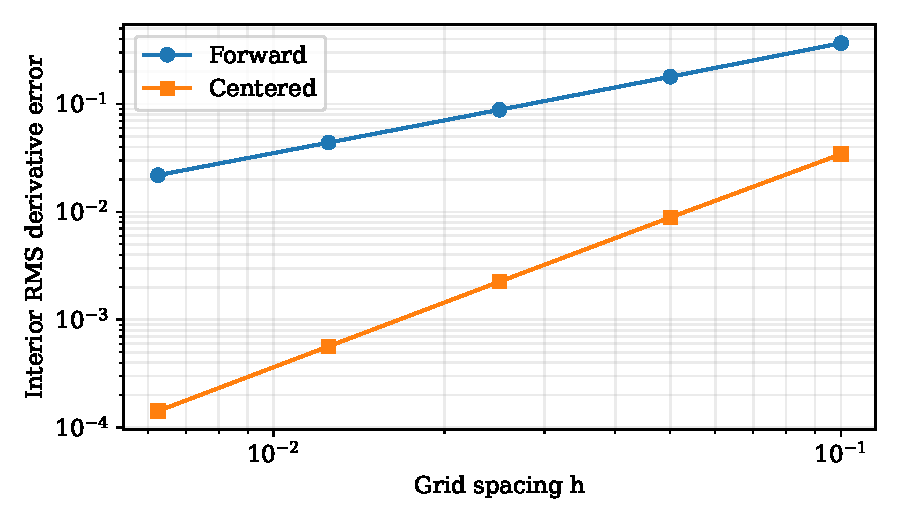
\includegraphics[width=.88\linewidth]{week01_assets/derivative_refinement.pdf}
\end{center}
{\small\textbf{Executed derivative check.} $f(x)=\sin(\pi x)$, $N=11,21,41,81,161$, $h=1/(N-1)$. Both methods are evaluated at interior nodes. The finest-pair observed orders are 1.005 (forward) and 1.995 (centered). This checks derivative accuracy; it does not establish cavity grid independence.}

\textbf{Predict, run, explain.} Before running, predict the factors of two and four for forward and centered errors. After running, explain why the observed orders approach one and two. The finest grid is not automatically exact; eventually floating-point cancellation can compete with truncation error.
\newpage
\topic{7.2}{The two-dimensional stencil and array slices}\label{sec:fd-grid}
A \textbf{stencil} is the set of nodes and weights used for one derivative approximation. The Laplacian $\nabla^2f=f_{xx}+f_{yy}$ adds the curvatures along the two coordinate directions. We write $f_{j,i}=f(x_i,y_j)$ because NumPy indexes rows ($y$) before columns ($x$), although coordinates are written $(x,y)$. At $(x_i,y_j)$, use two neighbors in $x$ and two in $y$. Equal spacing gives the five-point Laplacian. Diagonal nodes are not used by this stencil.
\begin{center}
\begin{tikzpicture}[x=1.5cm,y=1.05cm,>=stealth]
\draw[step=1,gray!35] (-1.1,-1.1) grid (1.1,1.1);
\draw[accent,thick] (-1,0)--(1,0) (0,-1)--(0,1);
\foreach \x/\y/\lab in {0/0/C,1/0/E,-1/0/W,0/1/N,0/-1/S}
{\node[draw=accent,fill=white,circle,inner sep=4pt] at (\x,\y) {$\lab$};}
\node[right] at (1.3,0) {$E=f_{j,i+1}$};
\node[above] at (0,1.25) {$N=f_{j+1,i}$};
\node[below] at (0,-1.25) {$S=f_{j-1,i}$};
\node[left] at (-1.3,0) {$W=f_{j,i-1}$};
\draw[->] (3,-1)--(3.6,-1) node[right] {$x,\ i$};
\draw[->] (3,-1)--(3,-.3) node[above] {$y,\ j$};
\end{tikzpicture}
\end{center}
\[
L_h f=\frac{E-2C+W}{\Delta x^2}+\frac{N-2C+S}{\Delta y^2}
\quad\xrightarrow{\Delta x=\Delta y=h}\quad
\frac{E+W+N+S-4C}{h^2}.
\]
\textbf{Numerical check.} For $f=x^2+3y^2$ at $(0.5,0.5)$ and $h=0.1$, $(C,E,W,N,S)=(1,1.11,0.91,1.33,0.73)$. Then $L_h f=(4.08-4)/0.01=8$, matching $f_{xx}+f_{yy}=2+6$. This smooth polynomial is a stencil check, not a cavity solution.

\textbf{One stencil, many nodes at once.} In an $N_y\times N_x$ NumPy array:
\begin{center}\begin{tabular}{lll}\toprule
Stencil part & Python slice & Shape\\\midrule
Center & \texttt{f[1:-1, 1:-1]} & $(N_y-2,N_x-2)$\\
East / west & \texttt{f[1:-1, 2:]} / \texttt{f[1:-1, :-2]} & Same\\
North / south & \texttt{f[2:, 1:-1]} / \texttt{f[:-2, 1:-1]} & Same\\\bottomrule
\end{tabular}\end{center}
\texttt{1:-1} excludes the first and last entries; \texttt{2:} starts at index 2; \texttt{:-2} stops before the last two entries. NumPy applies arithmetic element by element to these equally shaped blocks. For $N=65$, every interior block is $63\times63$.

\textbf{Read \texttt{laplacian(phi, dx, dy)}.} It allocates \texttt{zeros\_like(phi)}, fills only the interior using the two second differences, and returns an array of the original shape. Its zero boundary entries are uncomputed placeholders, not a claim that the physical Laplacian is zero at a wall. The transport function writes the same interior stencil explicitly.
\newpage
\topic{7.3}{From the Poisson stencil to a coupled system}\label{sec:fd-system}
For equal spacing, $L_h\psi=-\omega$ becomes
\[
4\psi_C-\psi_E-\psi_W-\psi_N-\psi_S=h^2\omega_C.
\]
Solving this row for $\psi_C$ gives a local update, but its four neighbors are also unknown. This is why discretization produces a \emph{system} of equations rather than a collection of independent calculations.

For unequal spacings, the same rearrangement gives
\begin{equation}
\psi_{j,i}^{k+1}=\frac{(\psi^k_{j,i+1}+\psi^k_{j,i-1})\Delta y^2+(\psi^k_{j+1,i}+\psi^k_{j-1,i})\Delta x^2+\omega_{j,i}\Delta x^2\Delta y^2}{2(\Delta x^2+\Delta y^2)}.
\end{equation}
Here $k$ counts inner sweeps; $\omega$ remains fixed throughout this Poisson solve.

\textbf{A four-unknown problem you can solve by hand.} Take two interior nodes in each direction in the unit square: $h=1/3$. All boundary values of $\psi$ are zero. Label the interior values $a,b$ along the lower row and $c,d$ along the upper row, and prescribe $\omega=-2$ at all four interior nodes. Then
\[
\begin{bmatrix}
4&-1&-1&0\\-1&4&0&-1\\-1&0&4&-1\\0&-1&-1&4
\end{bmatrix}
\begin{bmatrix}a\\b\\c\\d\end{bmatrix}
=-\frac{2}{9}\begin{bmatrix}1\\1\\1\\1\end{bmatrix}.
\]
The solution is $a=b=c=d=-1/9$. This example tests the Poisson equation only; its prescribed vorticity is not obtained from a complete no-slip cavity solve.

\textbf{Jacobi iteration from zero.} Update each node from the \emph{previous sweep's} neighbors:
\[
a^{k+1}=\tfrac14(b^k+c^k-2/9),\qquad
b^{k+1}=\tfrac14(a^k+d^k-2/9),
\]
with analogous rows for $c,d$. Symmetry makes all four entries identical in this example:
\begin{center}\begin{tabular}{rrr}\toprule
Sweep $k$ & Each interior $\psi$ & Error relative to $-1/9$\\\midrule
0 & $0$ & $1/9$\\
1 & $-1/18$ & $1/18$\\
2 & $-1/12$ & $1/36$\\
3 & $-7/72$ & $1/72$\\
$\infty$ & $-1/9$ & $0$\\\bottomrule
\end{tabular}\end{center}
\textbf{Why the code uses \texttt{old = psi.copy()}.} A complete snapshot makes the dependence on the old sweep explicit. In a nested point loop, immediately reusing updated neighbors would instead give a Gauss--Seidel-type sweep. In NumPy, the whole right-hand expression is evaluated before assignment, but \texttt{.copy()} also makes the algorithm unambiguous and preserves the earlier values.

This Poisson iteration index $k$ is not time. Its inputs are a fixed current $\omega$ and fixed wall $\psi$. After this solve, the outer algorithm evolves $\omega$ and must solve a new Poisson problem.

\checkpoint{Starting from zero, compute the first Jacobi sweep in the four-node example, then identify the matching array slices. Does doubling the number of inner sweeps advance physical time? No: it only improves the Poisson solve at fixed vorticity.}
